% noninjective.tex - standalone build of paper fig:noninjective
% (tikzpicture copied verbatim from paper/main.tex lines 359-423).
% Rebuild with: pdflatex noninjective.tex
\documentclass[tikz,border=6pt]{standalone}
\usetikzlibrary{arrows.meta}
\begin{document}
	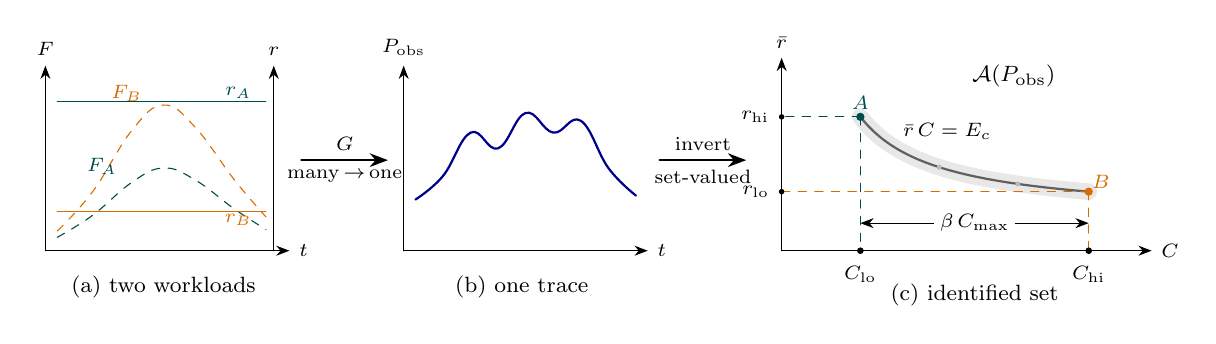
\begin{tikzpicture}[>=Stealth, line join=round, line cap=round]

		% ================= (a) two admissible workloads =================
		\begin{scope}[shift={(0,0)}]
			\draw[->] (0,0.55) -- (3.1,0.55) node[right] {\scriptsize $t$};
			\draw[->] (0,0.55) -- (0,2.9) node[above] {\scriptsize $F$};
			\draw[->] (2.9,0.55) -- (2.9,2.9) node[above] {\scriptsize $r$};
			\draw[teal!60!black] (0.15,2.45) -- (2.8,2.45);
			\draw[teal!60!black, dashed] plot[smooth, tension=0.7] coordinates
			{(0.15,0.72) (0.6,1.0) (1.1,1.42) (1.5,1.6) (1.9,1.45) (2.4,1.08) (2.8,0.82)};
			\draw[orange!85!black] (0.15,1.05) -- (2.8,1.05);
			\draw[orange!85!black, dashed] plot[smooth, tension=0.7] coordinates
			{(0.15,0.8) (0.6,1.3) (1.1,2.08) (1.5,2.4) (1.9,2.12) (2.4,1.45) (2.8,0.98)};
			\node[teal!60!black, anchor=south, inner sep=0.5pt] at (2.45,2.46) {\scriptsize $r_A$};
			\node[orange!85!black, anchor=north, inner sep=0.5pt] at (2.45,1.04) {\scriptsize $r_B$};
			\node[teal!60!black, anchor=east, inner sep=1pt] at (0.95,1.62) {\scriptsize $F_A$};
			\node[orange!85!black, anchor=south east, inner sep=0.5pt] at (1.25,2.42) {\scriptsize $F_B$};
			\node[anchor=north] at (1.5,0.35) {\footnotesize (a) two workloads};
		\end{scope}

		\draw[->, thick] (3.25,1.7) -- (4.35,1.7);
		\node[anchor=south, inner sep=1pt] at (3.8,1.78) {\scriptsize $G$};
		\node[anchor=north, inner sep=1pt] at (3.8,1.62) {\scriptsize many$\,\to\,$one};

		% ================= (b) one power trace =================
		\begin{scope}[shift={(4.55,0)}]
			\draw[->] (0,0.55) -- (3.1,0.55) node[right] {\scriptsize $t$};
			\draw[->] (0,0.55) -- (0,2.9) node[above] {\scriptsize $P_{\mathrm{obs}}$};
			\draw[thick, blue!55!black] plot[smooth, tension=0.7] coordinates
			{(0.15,1.2) (0.5,1.5) (0.85,2.05) (1.2,1.85) (1.55,2.3)
				(1.9,2.05) (2.25,2.2) (2.6,1.6) (2.95,1.25)};
			\node[anchor=north] at (1.5,0.35) {\footnotesize (b) one trace};
		\end{scope}

		\draw[->, thick] (7.8,1.7) -- (8.9,1.7);
		\node[anchor=south, inner sep=1pt] at (8.35,1.78) {\scriptsize invert};
		\node[anchor=north, inner sep=1pt] at (8.35,1.62) {\scriptsize set-valued};

		% ================= (c) identified set = constant-energy arc =================
		\begin{scope}[shift={(9.35,0)}]
			\draw[->] (0,0.55) -- (4.7,0.55) node[right] {\scriptsize $C$};
			\draw[->] (0,0.55) -- (0,3.0) node[above] {\scriptsize $\bar r$};
			\draw[line width=6pt, gray!18, line cap=round, smooth, samples=60, domain=1.0:3.9]
			plot (\x,{1.2776/\x+0.9724});
			\draw[gray!75!black, thick, smooth, samples=60, domain=1.0:3.9]
			plot (\x,{1.2776/\x+0.9724});
			\node[anchor=south west, inner sep=1pt] at (1.5,1.92) {\scriptsize $\bar r\,C=E_c$};
			\node[anchor=south] at (2.95,2.5) {\footnotesize $\mathcal{A}(P_{\mathrm{obs}})$};
			\fill[gray!55] (2.0,1.611) circle (0.9pt);
			\fill[gray!55] (3.0,1.398) circle (0.9pt);
			\fill[teal!60!black]   (1.0,2.25) circle (1.5pt) node[above, inner sep=2.5pt] {\scriptsize $A$};
			\fill[orange!85!black] (3.9,1.3)  circle (1.5pt) node[above right, inner sep=1pt] {\scriptsize $B$};
			\draw[dashed, teal!60!black]   (1.0,2.25) -- (0,2.25);
			\draw[dashed, orange!85!black] (3.9,1.3)  -- (0,1.3);
			\fill (0,2.25) circle (1.0pt) node[left=1pt] {\scriptsize $r_{\mathrm{hi}}$};
			\fill (0,1.3)  circle (1.0pt) node[left=1pt] {\scriptsize $r_{\mathrm{lo}}$};
			\draw[dashed, teal!60!black]   (1.0,2.25) -- (1.0,0.55);
			\draw[dashed, orange!85!black] (3.9,1.3)  -- (3.9,0.55);
			\fill (1.0,0.55) circle (1.2pt) node[below=2pt] {\scriptsize $C_{\mathrm{lo}}$};
			\fill (3.9,0.55) circle (1.2pt) node[below=2pt] {\scriptsize $C_{\mathrm{hi}}$};
			\draw[<->] (1.0,0.9) -- (3.9,0.9) node[midway, fill=white, inner sep=2pt] {\scriptsize $\beta\,C_{\max}$};
			\node[anchor=north] at (2.45,0.25) {\footnotesize (c) identified set};
		\end{scope}

	\end{tikzpicture}
\end{document}
